\documentclass[preprint, 10pt]{sigplanconf}
\usepackage{url}
\usepackage{amsmath}
\usepackage{booktabs}
\usepackage{longtable}
\usepackage{tikz}
\usepackage{listings}
\usetikzlibrary{positioning}
\newcommand{\cL}{{\cal L}}
\newcommand{\colAwidth}{0.1\textwidth}
\newcommand{\colBwidth}{0.34\textwidth}
\begin{document}

\special{papersize=8.5in,11in}
\setlength{\pdfpageheight}{\paperheight}
\setlength{\pdfpagewidth}{\paperwidth}

\conferenceinfo{Onward! '16}{October 30--November 4, 2016, Amsterdam, Netherlands}
\copyrightyear{2016}
\copyrightdata{978-1-nnnn-nnnn-n/yy/mm}
\copyrightdoi{nnnnnnn.nnnnnnn}

% Uncomment the publication rights you want to use.
%\publicationrights{transferred}
%\publicationrights{licensed}     % this is the default
%\publicationrights{author-pays}

\titlebanner{DRAFT -- Do not distribute}        % These are ignored unless
\preprintfooter{Paper submission for Onward! 2016}   % 'preprint' option specified.

\title{Be Consistent}
\subtitle{A Knowledge-Based Approach to Software Engineering}

\authorinfo{Omitted for Submission} %Dan Szymczak}
           {Omitted for Submission} %McMaster University}
           {Omitted for Submission} %szymczdm@mcmaster.ca}
\authorinfo{Omitted for Submission} %Jacques Carette\and Spencer Smith}
           {Omitted for Submission} %McMaster University}
           {Omitted for Submission} %carette@mcmaster.ca / smiths@mcmaster.ca}

\maketitle

\begin{abstract}
Every developer should aim to create high-quality software. In many instances,
software artifacts are not kept consistent or up-to-date. This lack of
consistency negatively impacts the overall quality of the software, particularly
its maintainability, traceability, and verifiability. We have combed through the
work of others to find ideas we believe will contribute to better consistency
and overall higher quality software. In combining these ideas, we have created a
knowledge-based approach for software development. We believe that if there is a
strong theoretical background in a given problem domain, and if it can be
effectively operationalized, then our method will lead to long-term improvements
in software quality for a (high) short-term investment. We have created a
framework (Drasil) to demonstrate these ideas.
\end{abstract}

%\category{CR-number}{subcategory}{third-level}

% general terms are not compulsory anymore,
% you may leave them out
%\terms
%term1, term2

\keywords
Literate software, knowledge capture, traceability, software engineering, scientific 
computing, artifact generation, software quality

\section{Introduction}
\label{sec:Intro}

We want to make better software.  In particular, we are interested in
increasing maintainability, traceability, reproducibility, verifiability, and
reusability.  Our approach is to invest (much) more in the short-term to provide
outstanding long-term benefits. This is the fundamental trade-off in %SS - I
                                %don't see the connection between these two sentences?
our work: we expect our methods to work very well for domains that are well
understood with known (but potentially enormous) design spaces.  We do not claim
to tackle areas of software development where agile methods are
well-suited.  But we firmly believe that there are domains -- such as
safety-critical applications -- where agile is not only ill-suited, it would be
downright unprofessional to use..

Rather than talk in vague generalities, we will pick Scientific Computation
(SC) for illustrative purposes throughout this paper.  But the fundamental
ideas (and, in fact, our framework) should be applicable to any software
domain which has well-established theoretical underpinnings, and a well
understood translation of the theory into effective code.  SC is particularly
well-suited as it is also replete with \emph{program families}.

We believe that Knuth's Literate Programming (LP)~\cite{Knuth1984} contains
some fundamental insights, but is too restricted (i.e. just to code).  Rather
than restrict LP to just source code, we want to apply it to all software
artifacts (requirements and design documents, source files, test cases, build
instructions, user manuals, etc.).  In other words, our basic starting points is
to ``chunk'' all aspects of the software construction process, and then weave the
actual artifacts from those chunks.  We will discuss the details of how we do this
in Section~\ref{sec:Drasil}.

The LP idea of putting everything into a single source file will not scale
in this way.  Instead, we introduce the idea of libraries of ``common knowledge''
for concepts which tend to re-occur.  A low-level example would be the units
from the Syst\`{e}me International (SI) Units as ``common knowledge,'' which really
ought to be defined only once, and then re-used.  A higher-level example would be
the various components of the theory of heat transfer, including the conservation
of energy equation.

We should make it clear that none of the individual ideas presented
in this paper are new.  Knuth himself
said that ``I have simply combined a bunch of ideas that have been in the air
for a long time'' when he coined LP~\cite{Knuth1984}. We are, however, taking these
ideas and re-assembling them in novel ways.  Our principal aim is not a new
software framework for doing literate software, but rather a framework which,
over the long term, will allow us to do our own work (largely in scientific
computation, but also in mechanized mathematics) much more effectively.  Our design
is thus largely example-driven; we indeed have an industrial client who is
partially funding
this work, with the common aim of reducing the long-term cost of re-certifying
SC software as fit-for-use for certain safety related %SS - the term safety
                                %critical seems to be reserved for software
                                %directly related to safety, like a real time control system 
applications.  While the details of re-certification are beyond the scope of this paper, they 
are never far from our minds as we design and implement our framework.

Others have done similar work (which we will get into in Section~\ref{sec:bg}),
but they did not achieve the results we are envisioning. They either set their
aims on other targets, spent too long creating a grand design and ended up
without any real, practical results, or they simply were not brave enough to
break things down into the smallest necessary chunks.

We believe that we have assembled the right ideas to achieve our vision.
The overall success or failure of our approach hinges on the idea of a stable,
well understood knowledge base. If such knowledge does not exist, or cannot be
adequately captured, our approach will not work.  Our claim is that there 
are areas of application where the knowledge not only exists, it can be adequately
captured and operationalized in very effective ways.

As it stands, we are following a (not so) humble, practical route to achieving our
goals and improving the overall quality of (some SC) software.

%SS - I like when papers have a roadmap of what is coming, but with the limited
%time we have, we can skip it this time around.

\section{Requirements and Inspiration}
\label{sec:bg}

As we mentioned previously, none of the ideas behind our approach are new. We
are going to take advantage of the excellent work done by many others.  Let us
first take a look at the current state of SC software development, then we will
discuss our goals and requirements, followed by the tools and techniques that
inspired us. Finally we will conclude this section by discussing which ideas we
intend to borrow and how we intend to bring everything together.

\subsection{The current state of SC software development}
\label{subsec:scdev}

Most developers in SC software tend to put an emphasis on their science and not on good
software development~\cite{Kelly2007}. 
Consequently these developers tend to use an agile
philosophy~\cite{AckroydEtAl2008, CarverEtAl2007, EasterbrookAndJohns2009,
Segal2005} or an amethododical~\cite{Kelly2013}, or a knowledge acquisition
driven~\cite{Kelly2015} process. These developers are scientists first and
foremost and they do not usually view rigid, process-heavy approaches
favourably~\cite{CarverEtAl2007}.

More than half of these scientists do not have a good understanding of software
testing~\cite{Merali2010}. In fact, there is very limited use of automated
testing for scientific software~\cite{PatrickEtAl2015} and quality
assurance has ``a bad name among creative scientists and
engineers''~\cite[p.~352]{Roache1998}.

Another problem in SC is that knowledge reuse is not fulfilling its potential.
For instance, for mesh generators a large number of similar programs have been
written. A survey~\cite{Owen1998} shows 81 different mesh generator packages,
with 52 of them generating triangular meshes, and 37 of these using the same
algorithm of Delaunay triangulation. %SS - I think the Owen reference is to a
                                %web-page that no longer exists.  We should
                                %probably find a better example in the future.

Tool use in SC software development is also limited, especially the use of
version control software~\cite{Wilson2006}.  However, some advanced methods and
techniques are being applied in SC.  For instance, code generation has been
successful in SC, but thus far the focus has been on the creation of only one
software artifact: the code. Examples include Gaussian
elimination~\cite{Carette2006}, ATLAS, Blitz++, Spiral,
FFT~\cite{KiselyovEtAl2004}, and FEniCS~\cite{LoggEtAl2012}.

The lack of emphasis on more artifacts is disadvantageous to SC software
developers. The value of documentation and a structured process is illustrated
by a survey of statistical software for
psychology~\cite{SmithEtAl2015-SS-TR,SmithEtAl2015SQJ}. A case study on the
impact of a rational document driven process for SC software was performed on
legacy software for thermal analysis of a fuel pin in a nuclear
reactor~\cite{SmithAndKoothoor2016, SmithEtAl2013}. The redeveloped version
discovered 27 issues, ranging from trivial to substantive, within the previous
documentation. If rational documentation were used more often, some previous
errors in scientific code may have been uncovered. Previous SC software failures
that might have benefited from a rational process include: the Sleipner A oil
rig collapse~\cite[p.~38]{OliveiraAndStewart2006}, molecular protein structure
retractions~\cite{Miller2006}, the Patriot missile
disaster~\cite[p.~36]{OliveiraAndStewart2006}, and seismic data
processing~\cite{HattonAndRoberts1994}.

\subsection{Goals and requirements for our approach}

The current state of SC software development informs our requirements. We want
to tackle many of the problems stated therein, without requiring scientists to
become professional software developers. Instead, we should simplify the
development process by allowing them to focus on the science.

First and foremost we want to improve software qualities, specifically
maintainability, traceability, reproducibility, verifiability, and reusability.
We believe the first step towards these improved qualities is a better
understanding of the underlying knowledge behind the software itself.

Being able to communicate this improved understanding is also necessary, as it
will help with maintainability, reproducibility, and more down the road.  This
requires ensuring that all software artifacts (requirements, design,
source code, etc.) are consistent and \emph{always} up to date.

If we can essentially \emph{force} the developer to always have consistent and up
to date artifacts, without impeding their ability to develop (or wasting their
time), then we believe we have already succeeded in improving the software. The
less time a developer needs to spend maintaining and updating software, the
more time they have to do other important things. 

We also want to avoid one of the most classical software engineering mistakes:
duplication. Knowledge should not be duplicated, regardless of how many times it
must be displayed. If we can capture knowledge in an appropriate manner, then we
can simply reuse that knowledge wherever necessary without needing to
reimplement it.

Finally, software (and results) should be reproducible. We want to ensure that
given all of the appropriate knowledge surrounding a piece of software,
scientists will be able to reproduce that piece of software and any results
obtained with it.

To tackle our requirements we need to understand what has come before.  This
includes (but is not limited to) methods for ensuring consistency across
software artifacts and work done in the field of reproducible research.  The
next section discusses an important tool for reproducible research: Literate
Programming.

\subsection{Literate Programming}
\label{subsec:lp}

Literate programming is a programming methodology that was introduced by Knuth.
The LP methodology changes the focus from writing programs that simply instruct
the computer on how to perform a task. Instead, the focus is on explaining
(\emph{to humans}) what we want the computer to do~\cite{Knuth1984}.

In a literate program, the documentation and source code are all kept together in
one source. Literate programs are developed by breaking down algorithms into
small, easy to understand parts referred to as
\emph{chunks}~\cite{JohnsonAndJohnson1997} or \emph{sections}~\cite{Knuth1984}.
These chunks are then explained, documented, and implemented in a way that
promotes understanding -- they are not necessarily written in the order that the
computer would read them, but rather a ``psychological
order''~\cite{PieterseKourieAndBoake2004}. To get the working source code for a
program written in the LP style, you run the \emph{tangle} process. Similarly,
to extract and typeset the documentation you run the \emph{weave} process.

LP has advantages beyond understandability. Using LP has been experimentally
found to lead to better consistency between code and
documentation~\cite{ShumAndCook1993}. While the program is being developed, the
documentation tends to be updated simultaneously as it surrounds the source
code. We should also keep in mind that proper, consistent documentation leads to
many advantages while developing or maintaining software~\cite{Hyman1990,
Kotula2000}. When documentation does not match the system, it is a major
detractor to software quality~\cite{Kotula2000, Thimbleby1986}. Taken together,
we can see how LP (when used properly) leads to more elegant, effective,
maintainable, and understandable code~\cite{PieterseKourieAndBoake2004}.

With all of the benefits of LP, it is fairly astounding that it has not been very
popular~\cite{ShumAndCook1993}.  However, there are a few successful examples of LP in
SC; two that come to mind are VNODE-LP~\cite{Nedialkov2006} and
``Physically Based Rendering: From Theory to
Implementation''~\cite{PharrAndHumphreys2004}. The latter being both a literate
program and textbook on the subject. Shum and Cook discuss the topic of LP's
lack of popularity and present the idea that it comes from two main
issues:

\begin{enumerate}
\item Output language / text processor dependency.
\item Lack of flexibility on what to present or suppress in the output.
\end{enumerate}

There have been attempts to address these issues. Many have focused on changing or
removing the output language or text processor dependency. For example CWeb (for
the C language), noweb (programming language independent), javadoc (for Java),
DOC++ (for C++), Doxygen (for multiple languages), and more. Many of these new
tools came with new and interesting features, examples include:

\begin{enumerate}
\item A ``What You See Is What You Get'' (WYSIWYG)
editor~\cite{FritzsonGunnarssonAndJirstrand2002}.
\item Graphicdoc rules (using a word processor to compose graphics in
LP)~\cite{ShumAndCook1993}.
\item Phantom abstracting~\cite{ShumAndCook1993}.
\item Movement away from the idea of ``one source''~\cite{Simonis2003}.
\end{enumerate}

The development of so many tools for LP has helped drive the understanding
behind exactly what LP tools should be doing. On the other hand, the multitude
of tools is preventing LP from becoming mainstream~\cite{Ramsey1994}. Nowadays,
however, we can see parts of LP becoming standard in certain domains (for
example: Haskell, Agda, and R support LP).

\subsection{Expanding LP: Literate Software}

A new methodology was proposed in 2002 by Al-Maati and Boujarwah called
``Literate Software Development'' (LSD). It was designed as a combination and
evolution of LP and Box Structure~\cite{Mills1986}. Box Structure
is the idea of views (system specifications, design, code) with each view being
an abstraction communicating the same information in different levels of detail,
for different purposes~\cite{AlMatiiAndBoujarwah2002}.

The main idea behind LSD was to overcome the disadvantages of LP and box
structure. These disadvantages included: the inability of LP to specify
interfaces between modules; the lack of ability to decompose boxes; a lack of
tools to support box structure~\cite{Deck1996}; a lack of ability to implement
the high-level analysis and design created using box structures.

WebBox, when implemented, expanded LP and box structures to include new chunk
types; the ability to refine chunks into more chunks (and eventually Java code);
the ability to specify interfaces and communication between boxes; and the
ability to decompose boxes at any level.

% SS - At some point we should contrast LSD with Drasil.

\subsection{Reproducible research} 
\label{subsec:rr}

The term ``reproducible research'' is typically used to mean embedding
executable code in research papers to allow readers to reproduce the
results described~\cite{SchulteEtAl2012}. Reproducibility of results is
fundamental to the idea of good science. %SS - I'm not sure this is the main
                                %thing that people mean when they say
                                %reproducible research

Gentleman and Temple Lang introduced a means for combining research reports with
the relevant code, data, etc. This is called a ``compendium'' and it
encapsulates the full work of the author, as opposed to just the publication
version of their work. It also allows the reader to re-run computations (while
explicitly showing the computational details)~\cite{GentlemanAndLang2012}. The
authors proposed that peer review and distribution of scientific work should be
done using compendia.

Several tools have been developed for reproducible research (Sweave, SASweave,
Statweave, Scribble, Org-mode, etc.) with the most popular being
Sweave~\cite{SchulteEtAl2012}.

\subsection{Bringing the ideas together}
\label{subsec:ideas}

LP brings many great ideas to the table for helping us keep our software
artifacts consistent. First off, we love the idea of chunks. However, to achieve
our goals we believe chunks should not be just pieces of code, but
representations of knowledge. If we can ``capture'' knowledge about a concept
within a chunk, then that knowledge can be reused readily. On that note, chunks
can also decrease the amount of duplication. If the knowledge regarding one
concept is stored in a chunk, we never need to duplicate it.

The knowledge we would like to store should help us increase the
verifiability of the program -- we should be able to see all of the assumptions
and derivations that the chunk relies on. As such, we want to be storing
specification-level knowledge, not code-level. If anything, we should be able to
easily get to a code-level representation from the higher level knowledge.

Making sure the developer always keeps their artifacts consistent is difficult
in the standard LP style. Documentation and chunks are kept together in one
source, but changing one does not necessarily mean the other will be updated
accordingly. As such, we want to ensure that all of our artifacts are being
automatically updated each time the knowledge base is updated. This
also brings us to the idea of traceability: we should (at all times) be able to
find where any concept or piece of code came from.

Instead of the previous \verb|tangle| and \verb|weave| processes, we want to
introduce the idea of recipes and a standard generator. Instead of having two
processes (one for documentation, one for source code) we effectively want to
have one recipe for each software artifact, all of which can be used by a single
standard generator. Recipes will allow us to trace exactly what knowledge is
coming from which sources, as well as allow us to reproduce any software
artifacts trivially. In fact, anyone with access to the recipes and knowledge
base should then also be able to reproduce these artifacts.

With the idea of chunks and recipes working together to create all of our
software artifacts, we can expect software that is much easier to maintain. All
of our artifacts will consistently be up to date.

\section{Drasil}
\label{sec:Drasil}

We are currently developing a framework called Drasil (shortened from
\emph{Yggdrasil} from Norse Mythology, which is also known as the \emph{world
tree}). To avoid getting lost in the design phase, we have opted to take a very
practical and example-driven approach in implementing Drasil. There are three
fundamental ideas behind our design thus far:

\begin{enumerate}
\item Organize the knowledge base -- We want a knowledge base that we can
structure conceptually (i.e. keep knowledge for a certain class of problems
together). This is where chunks come into play: each chunk encapsulates a single
piece of knowledge like a concept or a quantity. We want to keep knowledge in
the smallest possible pieces while simultaneously organizing it into knowledge
libraries.

\item Use recipes to create artifacts -- We can think of each artifact in our
software project as a different view of our knowledge base. We want to use
recipes to specify exactly what information from the knowledge base is necessary
for each artifact, and how that information should be displayed. For many
artifacts we would like to have a standard recipe which can be quickly
customized for the current problem, which is how we will avoid duplicating
knowledge.

\item Remove technology constraints -- We want to be able to create our software
without worrying about the underlying technical constraints of our display or
specification technology, programming language(s), etc. Anyone using Drasil
should be able to work with the knowledge base and their recipes, then simply
set their output technology and have the generator take care of all the
technical details.
\end{enumerate}

We argue that by implementing Drasil around these ideas, we will see drastic
improvements in software quality. In fact, using a generative approach we can
avoid certain problems altogether. One obvious and recurring problem that comes
to mind when upgrading software is ``feature creep'' or ``software
bloat''~\cite{AmselEtAl2011}. With Drasil, a software upgrade will actually be a
completely new piece of software that includes the previously desired
functionality as well as the new upgrades. We will discuss further improvements
in more detail after our example in Section~\ref{subsec:example}.

\subsection{Drasil's current implementation}
\label{subsec:current}

Fundamentally, Drasil must be able to capture knowledge and produce different
views of that knowledge. With our current implementation we have each individual
piece of knowledge as a named \emph{chunk}. We are then able to manipulate our
chunks through the use of a \emph{recipe}. Our \emph{generator} interprets the
recipes to produce the final desired view. This view represents one of the many
software artifacts mentioned in Section~\ref{sec:Intro}.

There are several varieties of named chunks. In fact, we have a hierarchy of
chunk types where each new chunk encapsulates more than the previous one(s) (see
Figure~\ref{fig:chunks} for an idea, the labels in parentheses are added
knowledge). The most basic \emph{chunk} represents a named piece of information.
Above that we have named \emph{concepts} which introduce some descriptive
information.

A \emph{quantity} is a concept that has a symbolic representation (we can refer
to it by either its name or symbol). In a similar vein are \emph{units}, 
%need something more here -- (which encapsulates the units 
%attached to aconcept)??
and \emph{relation chunks} (which add the idea of a relation between some other
pieces of knowledge).

In an SC context, most of the knowledge we work with is represented as a
quantity with some units, in other words a \emph{unital} chunk. Expanding on
that, we can actually calculate values for many of these unital concepts. As
such, we have \emph{equation chunks (EqChunks)} which allow us to capture the
equation along with everything else included in a unital chunk.

\begin{figure}
\begin{center}
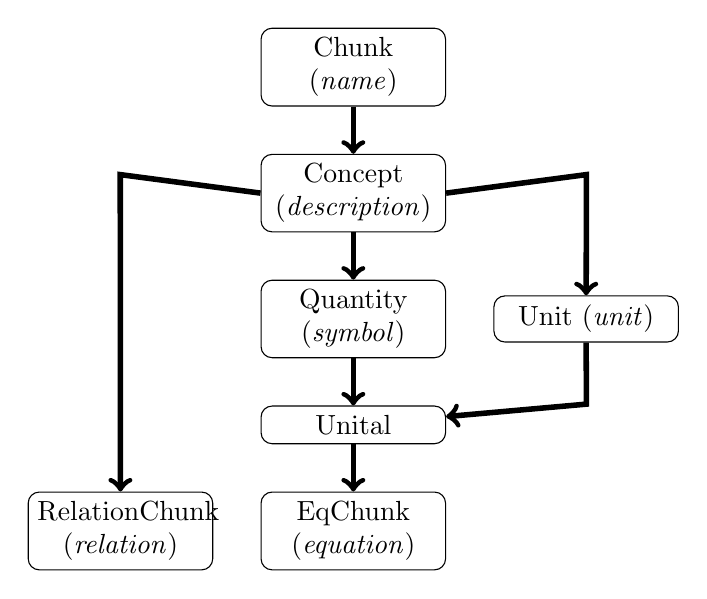
\begin{tikzpicture}[node distance=6mm]
  \tikzstyle{every node}=[draw,shape=rectangle, rounded corners,
    text width=6em, text centered];
  \node (ch)                     	{Chunk (\emph{name})};
  \node (co) [below = of ch]       {Concept (\emph{description})};
  \node (qu) [below = of co]  		{Quantity (\emph{symbol})};
  \node (u ) [right = of qu] 		{Unit (\emph{unit})};
  \node (uc) [below = of qu] 		{Unital};
  \node (eq) [below = of uc]	{EqChunk (\emph{equation})};
  \node (rc) [left = of eq]	{RelationChunk (\emph{relation})};

  \draw [->, line width=2pt] (ch) -- (co);
  \draw [->, line width=2pt] (co.west) -- (-2.96,-1.365) -- (rc); 
		%No idea how to do this
  \draw [->, line width=2pt] (co) -- (qu);
  \draw [->, line width=2pt] (co.east) -- (2.96,-1.365) -- (u );
  \draw [->, line width=2pt] (qu) -- (uc);
  \draw [->, line width=2pt] (u .south) -- (2.96,-4.28) -- (uc);
  \draw [->, line width=2pt] (uc) -- (eq);
\end{tikzpicture}
\end{center}
\caption{Our current chunk design (parentheses indicate newly added knowledge)}
\label{fig:chunks}
\end{figure}

Now with the means to encapsulate knowledge, we can turn our attention to our
recipes. The recipes are implemented using a combination of embedded Domain
Specific Languages (DSLs) in Haskell. We have currently implemented the
following DSLs:

\begin{enumerate}
\item Expression language -- A simple expression language that allows us to
capture knowledge relating to equations and mathematical operations. It includes
operations such as addition, multiplication, derivation, and exponentiation
among others.

\item Expression layout language -- A micro-scoped language for describing how
expressions should appear. Expressions may need to use a variety of inline
layout modifiers (subscripts, superscripts, etc.) to be properly displayed.

\item Document layout language -- A macro-scoped language for describing how
large-scale layout objects (tables, sections, figures, etc.) should appear.

\item C Representation Language -- A DSL for representing parts of the C
programming language inside the Drasil framework. This allows the generator to
produce working C code.

\item \LaTeX Representation Language -- A DSL for representing \LaTeX code
inside of Drasil. As with the C representation, it is used by the generator to
produce working \LaTeX code.

\item HTML Representation Language -- A DSL for representing HTML within Drasil.
Similar to the other representation languages as it is used by the
generator to produce working HTML.
\end{enumerate}

Of the DSLs mentioned, we actually only require three of them to write our
recipes. Each of the representation languages are used strictly by the generator
as an intermediary in the production of our desired views. We write our recipes
using the document layout language, expression layout language, and expression
language. We will discuss the particulars of each of these in more depth as part of
our example (Section~\ref{subsec:example}).

The last piece of the puzzle is the generator. We use it to interpret the
recipes, create intermediary representations of our desired views, and then
pretty-print them.

\subsection{Drasil in action} 
\label{subsec:example}

For this section we will take a look at a simplified version of a Software
Requirements Specification (SRS) for a fuel pin in a nuclear reactor (for more
information on that particular SRS see~\cite{SmithAndKoothoor2016}).

Starting off we will look at one specific term: $h_c$. In this example, $h_c$
represents the convective heat transfer coefficient between the clad and
coolant. The data definition for $h_c$ from the original SRS can be seen in
Figure~\ref{fig:h_c}.

\begin{figure}
~\newline \noindent \begin{minipage}{\textwidth}
\begin{tabular}{p{\colAwidth} p{\colBwidth}}
\toprule \textbf{Number} & \textbf{DD2 \label{hc}}
\\ \midrule 
Label & 
$h_{c}$
\\ \midrule
Units & $ML^0t^{-3}T^{-1}$\\ \midrule
SI Units & $\mathrm{\frac{kW}{m^{2o}C}}$\\ \midrule
Equation & $h_{c}$ =$
\frac{2k_{c}h_{b}}{2k_{c}+\tau_{c}h_{b}}$\\ \midrule
Description & $h_{c}$ is the convective heat transfer coefficient between clad
and coolant
\newline
$k_{c}$ is the
clad conductivity \newline
$h_{b}$ is the
initial coolant film conductance \newline
$\tau_{c}$ is the
clad thickness 
\newline
%NOTE: Equation taken from the code\\ \midrule  Sources & source code \\ \bottomrule 
\end{tabular} \end{minipage}\\ 
\caption{Data definition for $h_c$ from the fuel pin SRS}
\label{fig:h_c}
\end{figure}

The data definition of $h_c$ displays some interesting knowledge. It gives us
the name for a concept, its description, a symbol to use for easier reference,
its (SI) units, and its defining equation. Encapsulating all of this knowledge
into a chunk is not very difficult, as shown in Figure~\ref{fig:h_cChunk}. Note
that the equation for $h_c$ is written in our expression language (Expr) and it
also includes references to chunks that $h_c$ depends on. These will come into
play when we create the description for $h_c$ in the generated view, but we do
not concern ourselves with them now as their knowledge is stored elsewhere.
The units for $h_c$ are defined by a piece of common knowledge known as
\verb|heat_transfer|.

\begin{figure}
\begin{lstlisting}[frame=single, showstringspaces=false, basicstyle=\small]
h_c_eq :: Expr
h_c_eq = 2*(C k_c)*(C h_b) /
  (2*(C k_c) + (C tau_c)*(C h_b))

h_c :: EqChunk
h_c = fromEqn "h_c" 
 "convective heat transfer coefficient
    between clad and coolant"
 (sub h c) heat_transfer h_c_eq
\end{lstlisting}
\caption{The $h_c$ chunk in Drasil}
\label{fig:h_cChunk}
\end{figure}

On the topic of common knowledge, we can show an example alluded to previously,
that of the SI unit library. The seven base SI units captured in Drasil are
shown in Figure~\ref{fig:si_units}. The SI unit library also contains several
derived units (for example: Celsius which is derived from Kelvin) which we
make use of later on in our example. The knowledge behind each unit and (in the
case of derived units) their relation to the base units is captured in the
relevant chunks.

\begin{figure*}
\begin{lstlisting}[frame=single, showstringspaces=false]
metre, second, kelvin, mole, kilogram, ampere, candela :: FundUnit
metre    = fund "Metre"    "length (metre)"               "m"
second   = fund "Second"   "time (second)"                "s"
kelvin   = fund "Kelvin"   "temperature (kelvin)"         "K"
mole     = fund "Mole"     "amount of substance (mole)"   "mol"
kilogram = fund "Kilogram" "mass (kilogram)"              "kg"
ampere   = fund "Ampere"   "electric current (ampere)"    "A"
candela  = fund "Candela"  "luminous intensity (candela)" "cd"
\end{lstlisting}
\caption{The seven funamental SI Units in Drasil}
\label{fig:si_units}
\end{figure*}

Now that we've shown a bit of knowledge capture, you may be wondering how to use
it. This is where the recipes come in. Figure~\ref{fig:recipe} shows a portion
of the recipe for creating our intended SRS view. The body of the simplified SRS
is composed of three sections: \verb|s1|, \verb|s2|, and \verb|s3|. We then show
the definition of the first section (omitting the others for brevity) which is
titled "Table of Units" and includes an introductory paragraph and a table. This
table simply extracts the symbol and description information from the SI units
to display them in our view. It should be fairly obvious at this point, but
these macro-scale layout objects (sections, tables, paragraphs, etc.) are
specified using our document layout language.

\begin{figure}[tb]
\begin{lstlisting}[frame=single, 
  showstringspaces=false, basicstyle=\scriptsize]
srsBody = srs [h_g, h_c] "Spencer Smith" [s1,s2,s3]

s1 = Section (S "Table of Units") [intro, table]

table = Table 
 [S "Symbol", S "Description"] (mkTable
   [(\x -> Sy (x ^. unit)),
    (\x -> S (x ^. descr)) ] si_units)

intro = Paragraph (S "Throughout this ...")
\end{lstlisting}
\caption{A portion of our simplified SRS recipe}
\label{fig:recipe}
\end{figure}

With our recipe in place, we are now able to run it through the generator and
see what it spits out. We've included the three sections of this simplified SRS
in Appendix~\ref{appendix:SRS}, and what you see there is the typeset version of
the generated \LaTeX code. We are also able to output our view as an HTML
document (Figure~\ref{fig:HTML_s1}).

\begin{figure}
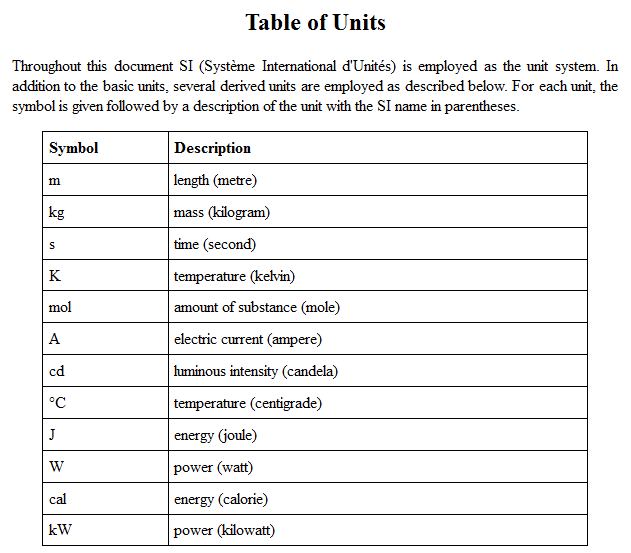
\includegraphics[scale=0.5]{HTML_s1.png}
\caption{Section 1 of the generated SRS (HTML version)}
\label{fig:HTML_s1}
\end{figure}

Now if you recall the data definition from Figure~\ref{fig:h_c}, we will show
the significant amount of work it takes to create (almost) that exact same
table: %SS - I think you are going for sarcasm here, but it doesn't come through
       %very well in written language.  Maybe you should add a smiley face, or
       %(sarcasm) in brackets?

\begin{lstlisting}
s3_dd2 = Definition (Data h_c)
\end{lstlisting}

Again looking to the appendix, or to the HTML output (Figure~\ref{fig:HTML_s3} for
the data definition), it should be easy to see that the recipe handled all of
the layout details. The recipe actually goes one step further in that it found
all of the chunk's dependencies and built the description by finding the
appropriate knowledge related to the other chunks. This is configurable in that
we can include short descriptions or verbose descriptions.

\begin{figure}
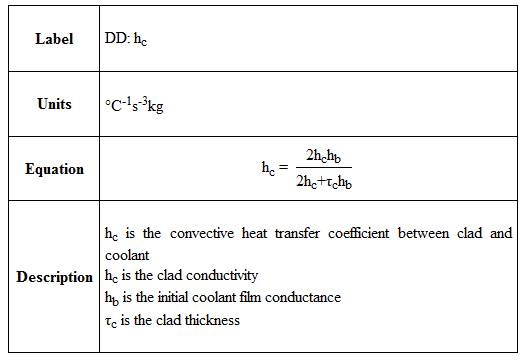
\includegraphics[scale=0.6]{HTML_s3.png}
\caption{Generated SRS data definition (HTML version)}
\label{fig:HTML_s3}
\end{figure}

One last thing we'd like to show is the source code generation. The recipe is
fairly straightforward in that we have:

\begin{lstlisting}[basicstyle=\small]
cSample = CodeBlock (toCode CLang Calc h_c)
\end{lstlisting}

All that says is \verb|cSample| is a block of code in the C language that
calculates the value of $h_c$. Currently the only implemented output language is
C, but we are planning to implement more and are designing around that coming
change. The generator output for \verb|codesample| ends up looking like:

\begin{lstlisting}[frame=single, 
  showstringspaces=false, basicstyle=\scriptsize]
double calc_h_c(double k_c, double h_b, double tau_c){
    return (2 * k_c * h_b / (2 * k_c + tau_c * h_b));
}
\end{lstlisting}

This is a fairly trivial piece of code, but it is a good example of how the
source can be generated from the high-level knowledge encapsulated in a chunk.

\subsection{Advantages}
\label{subsec:advantages}

We have already experienced some of the advantages of using Drasil. During the
knowledge capture phase of our example a seemingly trivial problem came up
regarding the simplified SRS. One of the concepts was being referred to with
multiple different descriptions. This led to an inconsistency in the
understandability of the document: a symbol represented ``description A'', then
halfway through the document the same symbol was explained as representing
``description B''. These descriptions were similar, but ``description B'' was
never used again. After capturing the (more) correct description, the generator
ensured internal consistency and the document was easier to understand. %SS - I don't
                                %entirely understand this example.  Could you be
                                %more specific?

With that in mind, look at all of the previous figures (or
Appendix~\ref{appendix:SRS}) and see how many times knowledge has been copied into
different places within one software artifact. Now imagine how many times that
knowledge appears across all software artifacts. By using a generator, we avoid
the problem of manually copying all of that information. It also ensures
that should a piece of knowledge need to be updated, those updates will
propagate throughout all of the artifacts \emph{automatically}.  This is how we
maintain consistency.
	%if this wasn't academia I would write ``automagically''
	
Another great benefit to knowledge capture, especially in the SC domain, is that
it promotes reuse. The SI units are a trivial example of a completely reusable
knowledge library that will come up across many different problem domains
(within and outside of SC). If we can build these common knowledge libraries for
a multitude of problem domains, we believe it will aid in the creation of higher
quality software overall and will allow developers and scientists to spend their
time on more important things, like their science.

Speaking of more important things, what about software certification? Many types
of safety- or security-critical software must be certified. Depending on the
certification process and regulatory body that means including different types
of high-quality documents along with the source code. As we all know,
requirements or algorithm choices can and do change throughout the software
development process leading to a need for updated documentation. With Drasil we
are able to ensure all of the software artifacts always remain consistent both
internally and with each other. %inter- and intra-artifact consistency

Drasil is meant to support design for change. We mentioned previously
(Section~\ref{sec:Intro}) that we intend to make working on program families
trivial, and Drasil does just that. Implementing a likely change is as simple as
adjusting a configuration file. If the knowledge has been properly captured, any
likely changes will involve trivial modifications. In the event of an unforeseen
change, modifying the recipe or (worse) the captured knowledge is still possible
and should end up simplifying the development process.

Finally, we need to verify our software and Drasil can help with that as well.
We can include so-called ``sanity'' checks in the knowledge we capture that can
be reused throughout the entire development process. A simple example of these
types of checks can be seen in the \verb|Constraints| column of
Table~\ref{tab:constraints}.

\begin{table} 
\centering
\nocaptionrule \caption{Constraints on quantities}
\begin{tabular}{|c|c|r|c|} \hline
\textbf{Var} & \textbf{Constraints} & \textbf{Typical Value} &
\textbf{Uncertainty}\\ \hline
$L$ & $L > 0$ & 1.5 m & 10\% \\ \hline
$D$ & $D > 0$ & 0.412 m & 10\% \\ \hline
$V_P$ & $V_P > 0$ & 0.05 m$^3$	& 10\% \\ \hline
$A_P$ & $A_P > 0$ & 1.2 m$^2$	& 10\% \\ \hline
$\rho_P$ & $\rho_P > 0$	& 1007 kg/m$^3$	& 10\% \\
\hline\end{tabular}
\label{tab:constraints}
\end{table}

If we encapsulate the knowledge regarding these constraints into the appropriate
chunks, we can have Drasil automatically test them for us. For example: a chunk
that contains the dimensions of a physical object should also constrain those
dimensions to positive values.

%SS - later we can add the example of testing for conservation of thermal energy

Another need in verification is traceability. With Drasil we have introduced
complete traceability: every piece of knowledge can be tracked (through all
software artifacts) to its source! We can also check that all chunks are
actually necessary, since the recipes can automatically report which chunks they
use.

With all knowledge coming from unique chunks, we get one last added benefit
(which can also be seen as a disadvantage): pervasive bugs. Any error in the
knowledge base will spread through every artifact and even a single bug could
break everything. However, we still see this as an advantage since the bugs tend
to be fairly shallow, easy to fix, and now much harder to miss.

\subsection{Disadvantages}
\label{subsec:disadvantages}

We mentioned one disadvantage in Section~\ref{sec:Intro}: the inability to
create a local hack to get things working. With Drasil we have to take an
all-or-nothing approach. This can, however, be viewed as an advantage: it
prevents the developer from adding undocumented knowledge to the project. Any
hacks added to the generated artifact sources will be overwritten the next time
anything is updated.

With an all-or-nothing approach we also remove the ability to iterate in a
meaningful way. We \emph{must} do everything right (or extremely close to it)
the first time. Yes, we can still modify the program family member that we are
generating and adapt as necessary, but adding new knowledge becomes a much
more involved process.

Adding new common knowledge libraries is also non-trivially difficult. These
must be created by (or with the help of) domain experts to ensure the right
knowledge is being captured in the right way.

\section{Future work}
\label{sec:fw}

Drasil is still in its early stages and currently is only producing one type of
code (in the C language) and one type of document (the SRS). However, we have
been greatly inspired and will continue to expand Drasil's implementation.
Currently, we plan to:

\begin{enumerate}
\item Generate code in more languages -- The next planned programming language
implementation is MATLAB, however, we plan to implement a variety of languages
as potential outputs.
\item Generate more artifact types -- We would like to see not only requirements
and code, but also test cases, design documents, build instructions, user
manuals and more! To do this we will be implementing new ``default'' recipes.
\item Generate different document views -- We are currently able to generate the
SRS with verbose or simplified data descriptions, but we would like to add a lot
more configurability to the view. For example: being able to have a view of the
requirements with full derivations of all equations from their sources vs.
having requirements that simply state the necessary equations to solve. Each
view is intended for a different audience.
\item More types of information in chunks -- See Table~\ref{tab:constraints} for
some ideas. We want to ensure we can encapsulate anything that comes our way.
\item Use constraints to generate test cases -- Typical values are considered
``reasonable'' values for realistic scenarios (if the user chooses values
outside of the ``reasonable'' range, warn them but do not stop them) whereas
physical constraints can be seen as hard limits on values (ex. density must
always be positive, otherwise throw an error).
\item Implement much larger examples -- We want to prove that Drasil can be
scaled up to usable examples and not just toy problems. At the time of this
writing, a larger example is currently being implemented. However, it is not
complete enough to show off (yet).
\item External syntax -- The current implementation of Drasil requires at least
  a basic understanding of Haskell syntax on top of each of the DSL's syntax. We
  would like to lower the barrier of entry by creating a singular external
  syntax to encompass all aspects of Drasil.
\end{enumerate}

\section{Concluding Remarks}
\label{sec:conclusion}

Many ideas are out there for improving the quality of software. We have proposed
a combination of these ideas which we believe will lead to vast improvements in
application domains where knowledge can adequately be captured and is well
understood.

With Drasil we hope to improve the qualities of traceability, maintainability,
and verifiability (among others) by leveraging a higher short-term investment
for long term gains. These gains can be most appreciated the longer a piece of
software is expected to be in use, especially when dealing with
(re-)certifiability and maintenance.

Drasil is already showing interesting results in its infancy. We hope to develop
it into a framework that can be used across many different problem domains with
many reusable common knowledge libraries.

\clearpage
\onecolumn
\appendix
\section{Simplified SRS}
\label{appendix:SRS}
Here we see the typeset output of the LaTeX code for the simplified SRS example:

\section*{Table of Units}
\label{Sec:ToU}
Throughout this document SI (Syst\`{e}me International
d'Unit\'{e}s) is employed as the unit system. In addition to
the basic units, several derived units are employed as
described below. For each unit, the symbol is given followed
by a description of the unit with the SI name in
parentheses.
\begin{longtable}{l p{8.5cm}}
Symbol & Description\
\\
m & length (metre)\
\\
kg & mass (kilogram)\
\\
s & time (second)\
\\
K & temperature (kelvin)\
\\
mol & amount of substance (mole)\
\\
A & electric current (ampere)\
\\
cd & luminous intensity (candela)\
\\
${}^{\circ}$C & temperature (centigrade)\
\\
J & energy (joule)\
\\
W & power (watt)\
\\
cal & energy (calorie)\
\\
kW & power (kilowatt)\
\\
\label{Table:ToU}
\end{longtable}
\section*{Table of Symbols}
\label{Sec:ToS}
The table that follows summarizes the symbols used in this document along with
their units. The choice of symbols was made with the goal of being consistent
with the nuclear physics literature and that used in the FP manual. The SI units
are listed in brackets following the definition of the symbol.
\begin{longtable}{l l p{8.5cm}}
Symbol & Description & Units\
\\
$h_{g}$ & effective heat transfer coefficient between clad
and fuel surface & ${}^{\circ}$C$^{-1}$s$^{-3}$kg\
\\
$h_{c}$ & convective heat transfer coefficient between clad
and coolant & ${}^{\circ}$C$^{-1}$s$^{-3}$kg\
\\
\label{Table:ToS}
\end{longtable}
\section*{Data Definitions}
\label{Sec:DD}
~\newline \noindent \begin{minipage}{.7\textwidth}
\begin{tabular}{p{0.2\textwidth} p{0.73\textwidth}}
\toprule \textbf{Refname} & \textbf{DD:h.g}
\label{DD:h.g}
\\ \midrule \\
Label & $h_{g}$
\\ \midrule \\
Units & ${}^{\circ}$C$^{-1}$s$^{-3}$kg
\\ \midrule \\
Equation & $h_{g}$ = $\frac{2h_{c}h_{p}}{2h_{c}+\tau{}_{c}h_{p}}$
\\ \midrule \\
Description & $h_{g}$ is the effective heat transfer
coefficient between clad and fuel surface
\\ \bottomrule \end{tabular}
\end{minipage}\\
~\newline \noindent \begin{minipage}{.7\textwidth}
\begin{tabular}{p{0.2\textwidth} p{0.73\textwidth}}
\toprule \textbf{Refname} & \textbf{DD:h.c}
\label{DD:h.c}
\\ \midrule \\
Label & $h_{c}$
\\ \midrule \\
Units & ${}^{\circ}$C$^{-1}$s$^{-3}$kg
\\ \midrule \\
Equation & $h_{c}$ = $\frac{2h_{c}h_{b}}{2h_{c}+\tau{}_{c}h_{b}}$
\\ \midrule \\
Description & $h_{c}$ is the convective heat transfer
coefficient between clad and coolant
\\ \bottomrule \end{tabular}
\end{minipage}\\

%\acks
%
%Acknowledgments, if needed.

% We recommend abbrvnat bibliography style.
\clearpage
\twocolumn

\bibliographystyle{abbrvnat}
\bibliography{drasil}
%
% The bibliography should be embedded for final submission.
%
%\begin{thebibliography}{}
%\softraggedright
%
%\bibitem[Smith et~al.(2009)Smith, Jones]{smith02}
%P. Q. Smith, and X. Y. Jones. ...reference text...
%
%\end{thebibliography}


\end{document}
